\documentclass[a4paper,11pt]{book}
\usepackage[utf8]{inputenc}
\usepackage{natbib}
\usepackage{url}
\setlength{\parskip}{12pt}
\usepackage{graphicx}

% Prepare the Python Code Display
\usepackage{listings}
\usepackage{color}

\definecolor{codegreen}{rgb}{0,0.6,0}
\definecolor{codegray}{rgb}{0.5,0.5,0.5}
\definecolor{codepurple}{rgb}{0.58,0,0.82}
\definecolor{backcolour}{rgb}{0.95,0.95,0.92}

\lstdefinestyle{Python}{
	backgroundcolor=\color{backcolour},   
	commentstyle=\color{codegreen},
	keywordstyle=\color{magenta},
	numberstyle=\tiny\color{codegray},
	stringstyle=\color{codepurple},
	basicstyle=\footnotesize,
	breakatwhitespace=false,         
	breaklines=true,                 
	captionpos=b,                    
	keepspaces=true,                 
	numbers=left,                    
	numbersep=5pt,                  
	showspaces=false,                
	showstringspaces=false,
	showtabs=false,                  
	tabsize=2
}

\lstset{style=Python}

\begin{document}
	
\frontmatter
\begin{titlepage}

\vspace*{40pt}

\begin{figure}
	\centering
	
\includegraphics[width=0.4\linewidth]{./Figures/Logo}
\end{figure}


\begin{center}
	
{\huge GWTSA User Manual V1.0}

\bigskip
{\Large R.A. Collenteur}

\bigskip

{\large July, 2015}

\end{center}


\vspace*{\fill}

\end{titlepage}
\section{Acknowledgements / Preface}
This piece of software is for a large part the result of the work on my Msc. thesis in 2014-2015 on non-linear time series analysis of groundwater levels. One of my goals during my thesis-period was to learn programming in python, a goal easily met with Mark Bakker as my supervisor. Somewhere halfway through the process, I realised how much time and effort had gone into programming, and the idea floated in my head of writing a python based software program that I could later share with others. As I think educating yourselves is part of your thesis, I took the opportunity to learn how to develop a software program and share it through Github. It meant that others would have to be able to read, work and make changes to my scripts. 'Acting' as if I was not going to be the only user of your script, really changed to way I did my programming.

However, apart from these personal incentives, I also had more fundamental reasons for starting this project. Firstly, as far as I am aware, there are no programs available that are completely open-source. Menyanthes is available on a commercial basis, and the Groundwater Statistics Toolbox by Peterson et al. [2014] requires Matlab. Secondly, you need complete control over the modelling process, which in my opinion is necessary for scientific work. While other software provides a graphical user interface (GUI), fast optimization and a great user experience, it is very difficult to change parameters, underlying assumptions or model structure. Especially the latter is important, as non-linear groundwater time series analysis requires a flexible model structure to implement the hydrologists system knowledge into the model, as I advocated in my thesis. Finally, the methods that I used in my study can be applied to other models without the user needing to write this piece of code all over again. 

GWTSA is an object-oriented program written in python. It allows the user to perform time series analysis of groundwater levels with just a few lines of code (Chapter3). Information on the model, its performance and the parameter estimation is easily accessed (chapter 4). However, the object oriented program structure also allows you to test new model structures, and a guide for adding new model structures is given in chapter 5. The software is envisioned for practical use, but also for more scientifically oriented projects. The scientific concepts that sit behind the model are discussed in-depth in chapters 6 and 7, as well as how these concepts are implemented in the model (chapter 8). It is tried to make to software as transparent as possible, so if anything is unclear don't hesitate to contact the author!

R.A. Collenteur [\url{info@raoulcollenteur.nl}]



 
\section{Changes Log}
\begin{itemize}
	\item{15th October 2015 - V0.0Alpha is released for testing and early case studies}
	\item{15th December 2015 - V0.0Beta is released after the thesis presentation}
\end{itemize}

\section{To Do:}

\begin{itemize}

\item{Check if climate time series are longer than groundwater time series at model setup}
\item{Check if units of the climate data are in the right order of magnitude}
\item{Calculate the water balance of the unsaturated zone and provide a method to check it}
\item{Add probability of exceedence graph}
\item{Transform parameter values back for reporting in plot\_results and plot\_diagnostics}
\item{Choose step at which innovations are taken into account not to on python index but real time value (Does this help on calibration?) }
\item{Make it possible to run without initial parameter estimates (maybe use a global optimization scheme then, and a local (fmin) otherwise?)}
\item{...}
\end{itemize}
\chapter{License}
GWTSA Software is published under a GNU GENERAL PUBLIC LICENSE. (?? At least private on Github for now..)
\tableofcontents
\mainmatter
\chapter{Introduction to GWTSA}
GWTSA stands for 'GroundWater Time Series Analysis' and is a Python base, open-source program to analyse and simulate time series of groundwater levels. This piece of software is intended for all of those interested in simulating groundwater levels through time series analysis, 

\section{What is Time Series Analysis?}

\section{What can it be used for?}


\chapter{Installation}

\subsection{Where to get GWTSA?}


\subsection{Installing on a Mac}

\subsection{Installing on Windows (Experimental)}

\subsection{Installing on other Operating Systems}

\subsection{Compiling the Unsaturated Zone Module using Cython}
The GWTSA software is unique in the point that it offers the ability to use a non-linear model to calculate the recharge. However, this comes at a price, most notably in terms of model complexity and computation times. The unsaturated zone model (captured in the python and cython files unsat\_zone.py/unsat\_zone.pyx) can increase the computation times dramatically and is therefore ported to a compiled language for increased performance in terms of computation speed. There is an interesting python package that can help in porting python code to compiled C-code: Cython (\url{http://cython.org}).

Cython can port pure python scripts to compiled C-code, but the speed-up will generally be limited to a few orders of magnitude (1-3 times as fast). A few modifications to your python script however, can eliminate bottlenecks and really boost the performance of your code. This cython-enhanced version of our python script is unsat\_zone.pyx, and is ready to be 'cythonized'. Cythonizing is the process of compiling your cython script to C-code and something that can than be imported back into your python scripts. On a mac, this means you create a Shared Object file, (unsat\_zone.so), and on windows you will create another file type (unsat\_zone.pyd). This means that the file extension is dependent on your operating systems and compiling the file needs to happen on the same operating system that GWTSA is used on. Compiling is straight forward and can be done following the following steps.

\textbf{On Mac OSX:}
\begin{itemize} 
\item{Open Terminal}
\item{Move to the directory where GWTSA is located using the 'cd' command (e.g. 'cd Projects/GWTSA')}
\item{Type 'python setup\_unsat\_zone.py build\_ext --inplace' and press Enter}
\item{Cython now compiled the code and a .so file is created. When available this .so file is automatically imported by python when importing GWTSA (Python import has a preferred order promoting compiled scripts if available) }
\item{\textbf{!!} It sometimes happens that the compiled .so file is put in a folder within the GWTSA folder, you should then move the unsat\_zone.so file to the GWTSA folder}
\end{itemize}

\textbf{On Windows:}
\begin{itemize} 
\item{Open command window (type 'CMD' in the start menu)}
\item{Move to the directory where GWTSA is located using the 'cd' command (e.g. 'cd Projects/GWTSA')}
\item{Type 'python setup\_unsat\_zone.py build\_ext --inplace' and press Enter}
\item{Cython now compiled the code and a .pyd file is created. When available this .pyd file is automatically imported by python when importing GWTSA (Python import has a preferred order promoting compiled scripts if available) }
\item{\textbf{!!} It sometimes happens that the compiled .pyd file is put in a folder within the GWTSA folder, you should then move the unsat\_zone.pyd file to the GWTSA folder}
\end{itemize}
\chapter{Setting up the model}
Setting up your first model in GWTSA is relatively simple, and can be done with just a few lines of code. However, before we dive into the actual code to run a model and analyse the results, let us quickly go over the structure of modelling in GWTSA. There are basically three phases that the user has to go through, as visualized in the flow diagram shown in figure \ref{GWTSA_Flow}. 

\begin{figure}[h]
\label{GWTSA_Flow}
\centering
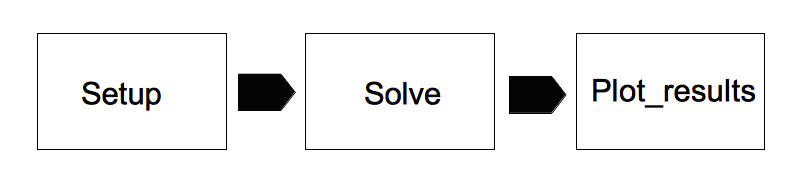
\includegraphics[width=1\linewidth]{Figures/GWTSA_Flow}
\caption{Flow diagram of the GWTSA modelling process}
\label{fig:GWTSA_Flow}
\end{figure}

In the first phase, an object is created for each borehole, and the necessary data is imported and prepared. This involved the determination of the time steps, model period etcetera. In the second phase, GWTSA performs the actual time series analysis and estimates the parameter values. It is in this phase that the model structure and important underlying assumptions can be chosen. The user is therefore encouraged to carefully read chapter 4 and choose the appropriate input arguments. The third phase is the analysis of th results, where GWTSA offers different graphs and numerics to interpret the model results.  

The first thing you want to do is open your python editor, and create a new .py file. The import of GWTSA can be done with the usual python import statements, if you have installed the software correctly. An example python file is available in the documentation folder to guide you through your first hands on experience. 

\section{Setup}
In this first phase the data necessary for a simulation is imported into an object. There are two important input files here: the observed groundwater levels and the climate data. Although the program is easy to adapt to your personal file format (simply change the np.loadtxt() input arguments), it is generally a good idea to use the input format similar to those in the Appendices of this manual. GWTSA will automatically select the right time steps, determine the model period and delete invalid observations from both time series. 

\textbf{Make sure to check the following:}
\begin{itemize}
\item{GWTSA expects a longer time series for the climate data than the groundwater data.}	
\item{The unit used throughout GWTSA is meters, so depending on the units of your input data, define by what value the data should be divided to get meters. Adapt input arguments `cl\_unit` and `gw\_unit` accordingly.}
\item{Set the right number of lines for both input files that GWTSA needs to skip when importing data using the 'rows' argument (groundwater and climate file respectively)}
\end{itemize}
	
\section{Solve}
Having set-up all the correct model data, a time series analysis can be performed by calling the 'solve' option. Here, there are two options that are important. The first is the model structure you want to use. Second, you need to provide a initial guess for the parameters, and here is where the hydrologists experience first enters the model. GWTSA can provide help on this, discussed in the next chapter 4. The software allows you to not provide a initial parameter estimate, but this is highly discouraged. The initial parameters need to be provided in a dictionary with parameter names that are similar as the model that is used. Although most of the parameter optimization is automatized, there are still many options available. To fully exploit these options read the advanced options section in chapter 4.

\textbf{Make sure to check the following:}
\begin{itemize}
	\item{Make sure the right parameters are provided in the dictionary}
	\item{Some of the parameters are scaled, take notice of this when providing the initial guess}
\end{itemize}

\section{Plot\_results}
Once we have estimated or optimized the parameters, we probably want to see what the resulting model looks like. We could run the simulate() function on our object, but the plot\_results function offers a neat way of simulating and viewing the resulting model. After running this function, the results window will pop up with a variety of information on your model. It combines different graphs of your data with the numerical values for some objective functions and the parameter values. This gives you the opportunity to visually check your model does what you expect it to do. 

\begin{figure}[h]
\centering
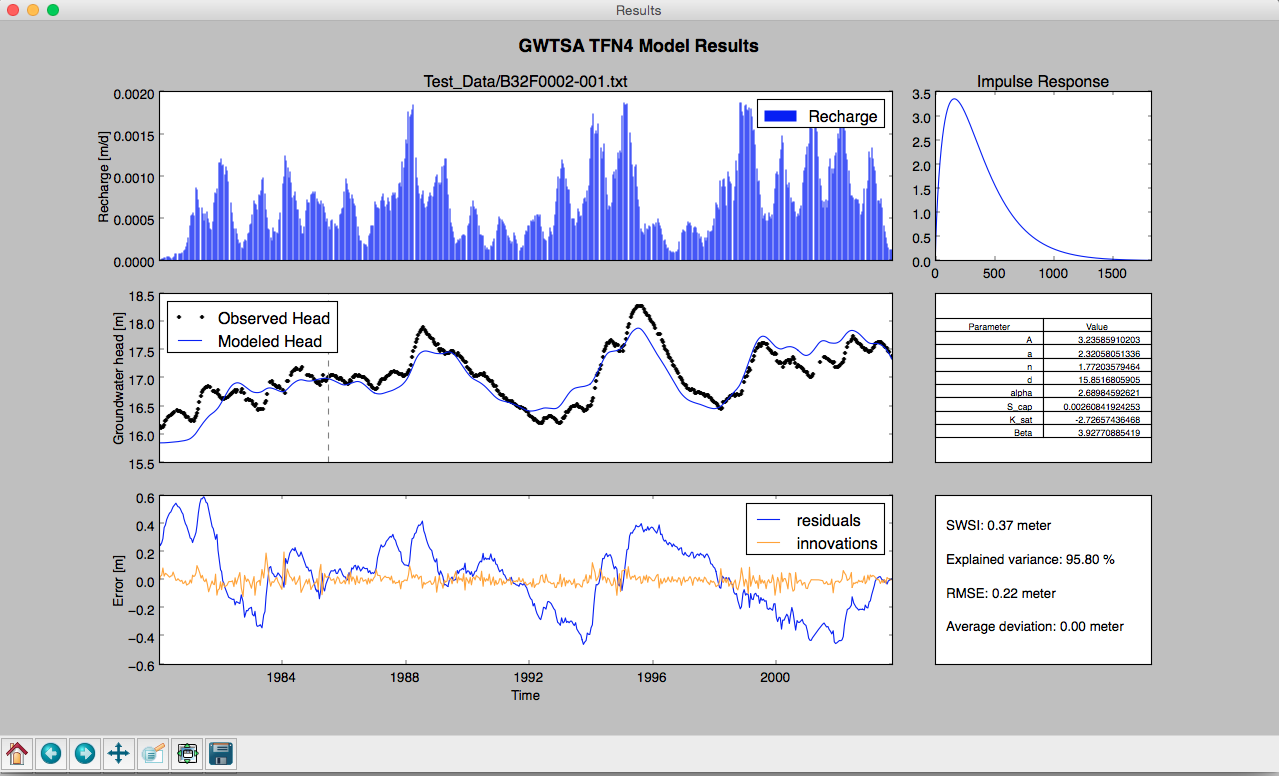
\includegraphics[width=1\linewidth]{Figures/plot_results}
\caption{Window showing the recharge, resulting model, model errors, impulse response shape and the parameter and objective function values}
\label{fig:plot_results}
\end{figure}


\section{Plot\_diagnostics}
It can sometimes be necessary to dive deeper into the parameter estimation process, to for example look at the evolution of the estimated parameter values or the correlation between parameters. Although it is always good to have a look at this window, it especially becomes useful when investigating new model structures. 

\begin{figure}[h]
\centering
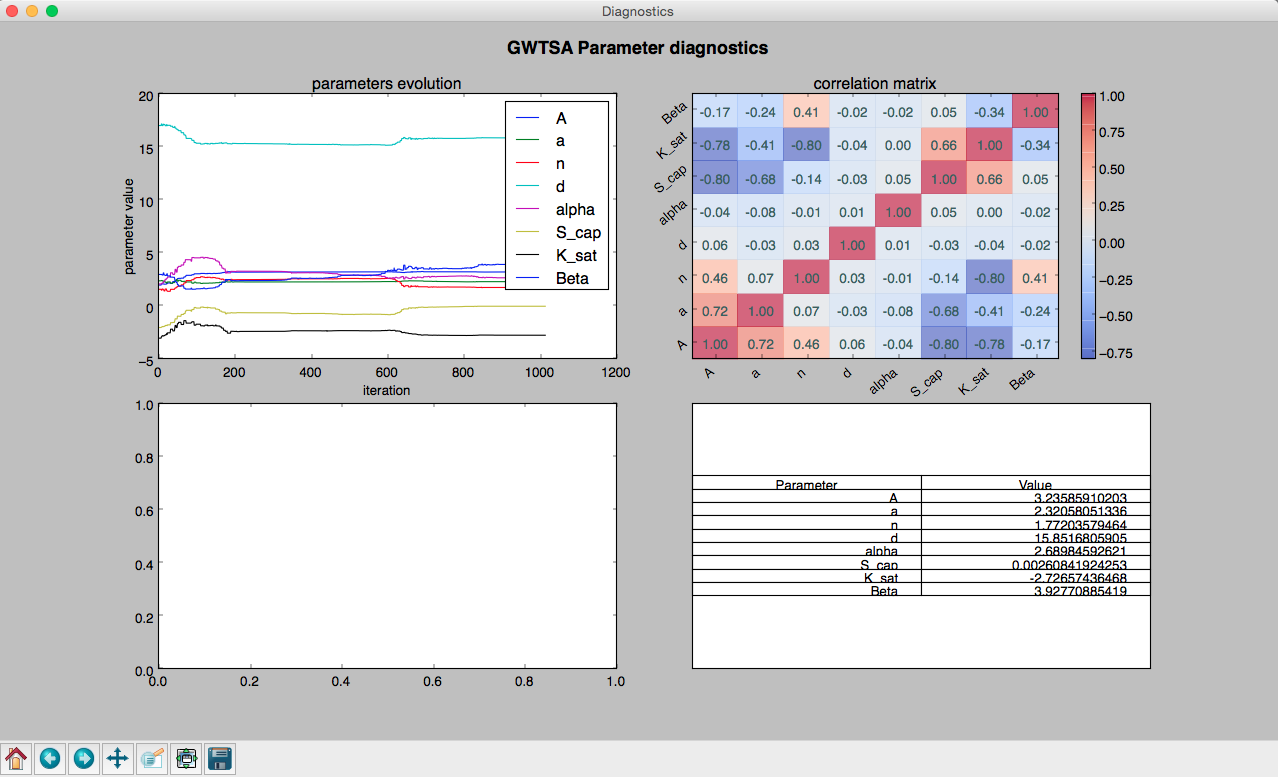
\includegraphics[width=1\linewidth]{Figures/plot_diagnostics}
\caption{Window showing the evolution of the parameters over the optimization, the correlation matrix and the final values for the parameters.}
\label{fig:plot_diagnostics}
\end{figure}

\section{Example script}
As stated in the introduction of this chapter, an entire simulation of GWTSA can be run with just a few lines of code. Below an example script to simulate the groundwater levels.

\begin{lstlisting}[language=Python]
from GWTSA import * 	# Import the entire GWTSA Toolbox

bore = 'Test_Data/GW_Levels.txt' #Groundwater Levels 
forcing = 'Test_Data/KNMI_Bilt.txt' # Climate Data
TFN = 'TFN4' # The Model structure

ts = Model(bore, forcing, rows=[5,8]) # Setup Phase

X0 = {'A': 3.0,'a': 2.2, 'n': 2.5,'Alpha': 10.0, 'S_cap': -1.00, 
		  'K_sat':-2.0, 'Beta': 3, 'D': -3, 'f': -0.1} 
		   # initial parameters as a dictionary

ts.solve(TFN, X0) # Solve Phase
ts.plot_results() # Results Phase
ts.plot_diagnostics() # Diagnostics Window
\end{lstlisting}

\chapter{Advanced GWTSA methods}

\section{Options for the Setup Function}

\textbf{Python code}
\begin{lstlisting}
ts.setup( 'GW_Levels.txt', 'Climate.txt', rows=[2,2], timestart=2000 gw_unit=1.0, cl_unit=10000.0)
\end{lstlisting}

\begin{itemize}
	\item{}
\end{itemize}



\section{Options for the Solve Function}

\textbf{Python code}
\begin{lstlisting}

X0 = {'A': 20,'a': 10, 'n': 1.5,'Alpha':40}
ts.solve('Nonlinear', X0, method=0)

\end{lstlisting}

\begin{itemize}
	\item{}
\end{itemize}

\section{Checking the Unsaturated Zone}


\include{./Theory}
\chapter{Implementation}

\section{Objective Function Revisited}
In this appendix it is shown that the modification proposed by \citet{peterson_nonlinear_2014} of the sum of weighted squared innovations (SWSI) objective function is mathematically similar to the original SWSI function introduced by \citet{von_asmuth_modeling_2005}. This function is defined as follows:

\begin{equation} \label{SWSI}
S^2(t,\beta) = \sum\limits_{j=1}^N \left\lgroup  \frac{ \sqrt[N]{ \prod\limits_{i=1}^N ( 1 - \exp^ \frac{-2 \Delta{t_i}}{\alpha} )  }}{ 1 - \exp^ \frac{-2 \Delta{t_j}}{\alpha} } \upsilon^2(\beta,t_j)    \right\rgroup
\end{equation}

When calibrating on long time series on with high frequency data, $N$ can become very large while the term $ 1 - \exp^( \frac{-2 \Delta{t_j}}{\alpha} $ becomes small. This can cause the product operator to near machine precision and return a value of 0.0 for the numerator. To solve this problem, \citet{peterson_nonlinear_2014} proposed to take the natural logarithm of $ { \sqrt[N]{ \prod\limits_{i=1}^N ( 1 - \exp^( \frac{-2 \Delta{t_i}}{\alpha} ) )  }} $

\begin{equation}
S^2(t,\beta) = \sum\limits_{j=1}^N \left\lgroup  \frac{ exp ^ { ln ({ \prod\limits_{i=1}^N ( 1 - \exp^ \frac{-2 \Delta{t_i}}{\alpha} )^ \frac{1}{N} ) } }}{ 1 - \exp^ \frac{-2 \Delta{t_j}}{\alpha} } \upsilon^2(\beta,t_j)    \right\rgroup
\end{equation}

which is essentially the same as \eqref{SWSI} when applying the mathematical rules $ ln(x^y) = y ln(x) $ and $ ln(ab) = ln(a) + ln(b) $. The final equation as proposed by \citet{peterson_nonlinear_2014} is then:

\begin{equation} \label{SWSI_adapted}
S^2(t,\beta) = \sum\limits_{j=1}^N \left\lgroup  \frac{ \frac{1}{N}{ \sum\limits_{i=1}^N ln( 1 - \exp^ \frac{-2 \Delta{t_i}}{\alpha} )  }}{ 1 - \exp^ \frac{-2 \Delta{t_j}}{\alpha} } \upsilon^2(\beta,t_j)    \right\rgroup
\end{equation}

As shown above, the two equations are mathematically similar. Numerically however, the adapted SWSI equation has a lower chance of running into machine precision causing calibration of the time series model to fail. Therefore, this equation is used as the objective function for parameter optimization. 


% In this section the numerical mathematics for solving the soil models is discussed. 
%
%


\section{Appendix B: Solving the Soil model}
In this appendix, the numerical mathematics that have been used to solve the unsaturated zone model are discussed. The unsaturated zone is described by a non-linear differential equation of which no analytical solution exists, and hence has to be solved numerically. Two different unsaturated zone models have been applied in this research. Below we will derive the numerical solution for the percolation model \eqref{percolation} in detail, while the solution of the piston flow model \eqref{pistonflow} is given and can be derived in a similar way.

\begin{equation} \label{percolation}
\frac{dS}{dt} = (P-I)- K_{sat}\left( \frac{S(t)}{S_{cap}}\right) ^\beta - E_p min(1, \frac{S}{0.5S_{cap}})
\end{equation}

\begin{equation} \label{pistonflow}
\frac{dS}{dt} = (P-I)(1-\left( \frac{S(t)}{S_{cap}}\right) ^\beta) - E_p min(1, \frac{S}{0.5S_{cap}})
\end{equation}

\citet{kavetski_calibration_2006-1} showed that for robust parameter optimization and calibration strategies, smoothness of the objective function is important. Therefore, the above equation is solved using the implicit Euler scheme. For simplicity in the following derivation, we define:

\begin{equation}
f(S,t) = (P-I)- K_{sat}\left( \frac{S(t)}{S_{cap}}\right) ^\beta - E_p min(1, \frac{S}{0.5S_{cap}})
\end{equation}

Applying the implicit Euler scheme gives the following:

\begin{equation}
\frac{S^{t+1}-S^t}{\Delta{t}} = f(S^{t+1})\\
\end{equation}
\begin{equation} \label{impeuler}
S^{t+1} = S^t + \Delta{t} * f(S^{t+1})
\end{equation}

This equation has to be solved iteratively, as $ S^{t+1} $ is unknown. The Newton-Raphson iteration method is used for this. Since the NR method is a root-finding technique that requires the form $ g(S^{t+1}) =0 $, we need to introduce a new equation for $  g(S^{t+1}) $ using equation \eqref{impeuler} :

\begin{equation}\label{g_function}
g(S^{t+1}) = S^{t+1} - S^t - \Delta{t} * f(S^{t+1}) = 0
\end{equation}

The equation for the Newton-Raphson iteration will than be:

\label{key}\begin{equation} \label{newtonraphson}
S^{t+1}_{i+1}=S^{t+1}_{i} - \frac{g(S^{t+1}_{i})}{g^{\prime} (S^{t+1}_{i})}
\end{equation}

The subscript $ i $ is the index for the iteration, hence every iteration the estimate of $ S^{t+1} $ is updated. For the first iteration, this requires an initial estimate of $ S^{t+1} $, in this study given applying an explicit euler scheme to solve equation \eqref{percolation} (no derivation given here). The derivative of $ g(S_i^{t+1}) $ depends on the system state, as $f(S,t)$ is not a continuous function:

\begin{equation}
g^{\prime} (S^{t+1}_{i}) = \frac{dg_{i}^{t+1}}{dS^{t+1}}
\end{equation}

\begin{equation}
g^{\prime} (S^{t+1}_{i}) =
\begin{cases}

1 - \Delta{t} \left\lgroup {  - K_{sat} \beta (\frac{S_i}{S_{cap}}) ^ {\beta-1}  } \right\rgroup 		& \text{if } S^{t+1}_{i}) >= 0.5 S_{cap} \\

1 - \Delta{t} \left\lgroup {  - K_{sat} \beta (\frac{S_i}{S_{cap}}) ^ {\beta-1}  - E_p  \frac{1}{0.5 S_{cap}} } \right\rgroup       & \text{if } S^{t+1}_{i}) < 0.5 S_{cap}
\end{cases}
\end{equation}

The superscript $ t+1 $ has been omitted from E and $ S_i $ for reasons of readability. Equation \eqref{newtonraphson} is generally solved within 3-5 iterations, depending on the error $\varepsilon $ that is allowed. However, in some cases the NR method does not find the solution and provides an error in the model. One of these errors is called the zero-division error and results from a value of the derivative that is (very close to) zero. Therefore, if this situation occurs, equation \eqref{g_function} is solved using the computationally more expensive bisection method for that specific time step.

The derivative $g^{\prime}$ for the piston flow model \eqref{pistonflow} is as follows:

\begin{equation}
g^{\prime} (S^{t+1}_{i}) =
\begin{cases}

1 - \Delta{t} \left\lgroup {  - (P-I) \beta (\frac{S_i}{S_{cap}}) ^ {\beta-1}  } \right\rgroup 		& \text{if } S^{t+1}_{i}) >= 0.5 S_{cap} \\

1 - \Delta{t} \left\lgroup {  - (P-I) \beta (\frac{S_i}{S_{cap}}) ^ {\beta-1}  - E_p  \frac{1}{0.5 S_{cap}} } \right\rgroup       & \text{if } S^{t+1}_{i}) < 0.5 S_{cap}
\end{cases}
\end{equation}

The recharge for percolation and the piston flow model is now calculated by numerical integration as:

\begin{equation}
R^{t+1} = K_{sat} \frac{\Delta t}{2}\left(\frac{S^t + S^{t+1}}{S_{cap}}\right)^\beta
\end{equation}

\begin{equation}
R^{t+1} = (P^{t+1}-I) \frac{\Delta t}{2}\left(1-\left(\frac{S^t + S^{t+1}}{S_{cap}}\right)^\beta\right)
\end{equation}
\chapter{Appendices}

\subsection{A: Example File Forcing input format}


\begin{lstlisting}
# This is an example file format. The second column contains the date, the third the precipitation and the fourth the potential evapotranspiration
# STN,YYYYMMDD,   RH, EV24
260,19621005,    2,   17
260,19621006,    0,   11
260,19621007,    1,   19
260,19621008,    1,   18
260,19621009,    0,   17

\end{lstlisting}

\subsection{B: Example File Observed Head input format}

\begin{lstlisting}
# This is an example file format of the observed heads. The first column contains the date and the second the measured heads in meters. 
#YYYYMMDD, GWL 
19800102,6.9995402504
19800114,7.11586624929
19800128,7.19826247613
19800214,7.24205916302
19800228,7.25891807093

\end{lstlisting}

\backmatter
\bibliography{main}

\end{document}